\documentclass{article}
\usepackage[utf8]{inputenc}
\usepackage[margin=1in]{geometry}

\title{452 - Midterm 1}
\author{Victor Zhang}
\date{March 2, 2021}

\usepackage[utf8]{inputenc}
\usepackage{amsmath}
\usepackage{amsfonts}
\usepackage{natbib}
\usepackage{graphicx}
% \usepackage{changepage}
\usepackage{amssymb}
\usepackage{xfrac}
% \usepackage{bm}
% \usepackage{empheq}
\usepackage{tikz}
\usepackage{tikz-qtree}
\usepackage{caption}
\usepackage{subcaption}
\usetikzlibrary{arrows,automata}
\usepackage{dirtytalk}


\newcommand{\contra}{\raisebox{\depth}{\#}}

\newenvironment{myindentpar}[1]
  {\begin{list}{}
          {\setlength{\leftmargin}{#1}
          \setlength{\rightmargin}{#1}}
          \item[]
  }
  {\end{list}}

\pagestyle{empty}

\begin{document}

\maketitle
% \begin{center}
% {\huge Econ 482 \hspace{0.5cm} HW 3}\
% {\Large \textbf{Victor Zhang}}\
% {\Large February 18, 2020}
% \end{center}

\section{}
\textit{On my honor, I have neither received nor given any unauthorized assistance on this examination.}

\section{}
We first show $(ab^* \cup b)^* = (a \cup b)^*$. Since the latter contains every possible string within $\Sigma^*$, it suffices to show $(ab^* \cup b)^* \supseteq (a \cup b)^*$. Indeed, since $a \subseteq ab^*$, $(a \cup b)^* \subseteq (ab^* \cup b)^*$, as desired. A minimal DFA must contain at least 3 states, since the language must contain at least 2 symbols $a$. We also need an absorbing state to handle input $b$ from the start state:

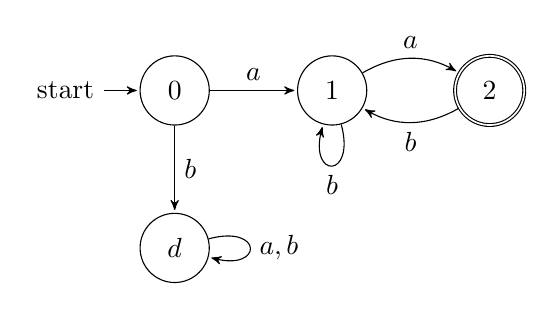
\begin{tikzpicture}[->,>=stealth',shorten >=1pt,auto,node distance=2cm,
        scale = 1,transform shape]

  \node[state,initial] (0) {$0$};
  \node[state] (1) [right of=0] {$1$};
  \node[state,accepting] (2) [right of=1] {$2$};
  \node[state] (d) [below of=0] {$d$};

  \path (0) edge              node {$a$} (1)
        (1) edge [bend left]  node {$a$} (2)
        (1) edge [loop below] node {$b$} (1)
        (2) edge [bend left]  node {$b$} (1)
        (0) edge              node {$b$} (d)
        (d) edge [loop right] node {$a,b$} (d);

\end{tikzpicture}

\section{}
\begin{figure}[!h]
  \begin{subfigure}[h]{0.4\textwidth}
    \centering
    \begin{tabular}{|*6{c|}}
    \cline{1-1}
    $S$&\multicolumn{4}{c}{}\\
    \cline{1-2}
    $A$&&\multicolumn{3}{c}{}\\
    \cline{1-3}
    &$C$&$B$&\multicolumn{2}{c}{}\\
    \cline{1-4}
    &&$C$&&\multicolumn{1}{c}{}\\
    \cline{1-5}
    $A$&&&$A$&$B$\\
    \cline{1-6}
    $B$&$C$&$B$&$B$&$C$&$A$\\
    \hline
    b&c&b&b&c&a\\
    \end{tabular}
  \end{subfigure}
  \hfill
  \begin{subfigure}[h]{0.4\textwidth}
    \centering
    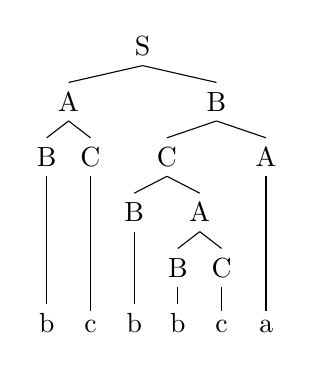
\begin{tikzpicture}
    \tikzset{level distance=20pt}
    \tikzset{frontier/.style={distance from root=100pt}}
    \Tree [.S
            [.A
              [.B b ]
              [.C c ]
            ]
            [.B
              [.C
                [.B b ]
                [.A
                  [.B b ]
                  [.C c ]
                ]
              ]
              [.A a ]
            ]
          ]
    \end{tikzpicture}
  \end{subfigure}
  \caption{bcbbca}
\end{figure}
\begin{figure}[!ht]
  \begin{subfigure}[h]{0.4\textwidth}
    \centering
    \begin{tabular}{|*6{c|}}
    \cline{1-1}
    $S$&\multicolumn{4}{c}{}\\
    \cline{1-2}
    &$B$&\multicolumn{3}{c}{}\\
    \cline{1-3}
    &$C$&&\multicolumn{2}{c}{}\\
    \cline{1-4}
    $S$&&&&\multicolumn{1}{c}{}\\
    \cline{1-5}
    &$B$&$S$&$A$&$B$\\
    \cline{1-6}
    $A$&$C$&$A$&$B$&$C$&$A$\\
    \hline
    a&c&a&b&c&a\\
    \end{tabular}
  \end{subfigure}
  \hfill
  \begin{subfigure}[h]{0.4\textwidth}
    \centering
    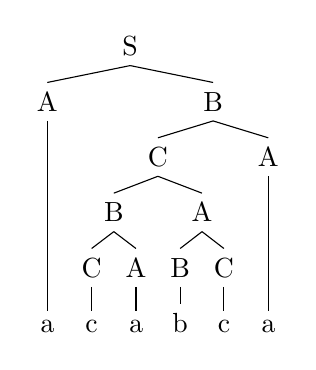
\begin{tikzpicture}
    \tikzset{level distance=20pt}
    \tikzset{frontier/.style={distance from root=100pt}}
    \Tree [.S
            [.A a ]
            [.B
              [.C
                [.B
                  [.C c ]
                  [.A a ]
                ]
                [.A
                  [.B b ]
                  [.C c ]
                ]
              ]
              [.A a ]
            ]
          ]
    \end{tikzpicture}
  \end{subfigure}
  \caption{acabca}
\end{figure}

\section{}
\begin{equation*}
\begin{cases}
S \to aBCd\\
B \to C \;|\; CBB\\
C \to \epsilon \;|\; da
\end{cases}
\to
\begin{cases}
S \to GH\\
G \to AB\\
H \to CD\\
B \to C \;|\; CBB\\
C \to \epsilon \;|\; DA\\
A \to a\\
D \to d\\
\end{cases}
\to
\begin{cases}
S \to GH\\
G \to AB\\
H \to d \;|\; JD\\
J \to DA\\
B \to \epsilon \;|\; BB \;|\; DA \;|\; DABB\\
A \to a\\
D \to d\\
\end{cases}
\to
\begin{cases}
S \to GH\\
G \to a \;|\; AB\\
H \to d \;|\; JD\\
J \to DA\\
B \to BB \;|\; DA \;|\; JK\\
K \to BB\\
A \to a\\
D \to d\\
\end{cases}
\end{equation*}

\section{}
For given $x,y$ we determine if the set of $z$ s.t. $xz,xy$ are both in or not in the language is $\Sigma^*$. If it is, $x \equiv_A y$.
\subsection{}
We note for all $z \in A$, $00z \in A$ and $000z \in A$. If $z \notin A$ it must contain either multiple 1s or a 0 after a 1. In both cases, $00z$ and $000z$ are both not in the language. Thus $00 \equiv_A 000$ $\Box$
\subsection{}
Take $z = 1$. Then $001 \in A$ but $00011 \notin A$. Thus $00 \not\equiv_A 0001$ $\Box$
\subsection{}
Both strings are in the language, and adding anything to the end generates something not in the language. Thus $00001 \equiv_A 0001$ $\Box$
\subsection{}
Take $z = \epsilon \in \Sigma^*$. $00001 \in A$ but $00011 \notin A$ so $00001 \not\equiv_A 00011$ $\Box$
\subsection{}
Suppose it is possible. Then it must accept $00$, accept $000$, accept $0001$, and reject $00010$. From the first two accepting states, the singular accepting state must have a self-transition 0. From the second and third accepting state, it must also have a self-transition 1. But from the last rejecting state, it must not have a self-transition 0, a contradiction $\contra$
\subsection{}
Yes, such an NFA is given:

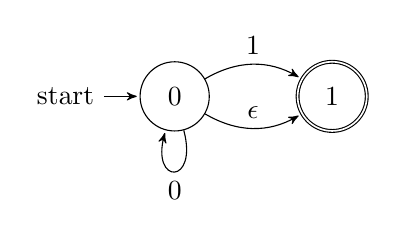
\begin{tikzpicture}[->,>=stealth',shorten >=1pt,auto,node distance=2cm,
        scale = 1,transform shape]

  \node[state,initial] (0) {$0$};
  \node[state,accepting] (1) [right of=0] {$1$};

  \path (0) edge [loop below] node {$0$} (0)
        (0) edge [bend right] node {$\epsilon$} (1)
        (0) edge [bend left]  node {$1$} (1);

\end{tikzpicture}

\section{}
There are multiple derivations for 0. Two possible derivations are
$$S \to AB \to \epsilon B \to 0B \to 0\epsilon = 0$$
$$S \to AB \to A \epsilon \to 0A \to 0\epsilon = 0$$
We note the grammar generates all strings $s \in \Sigma^*$, so it suffices to give a grammar that generates $\Sigma^*$:
\begin{equation*}
S \to \epsilon \;|\; 1S \;|\; 0S\\
\end{equation*}

\section{}
\subsection{}
We may write all (nonnegative) powers of 2 as $0^*10^*$, which is clearly \textbf{regular} and accepted by the NFA:

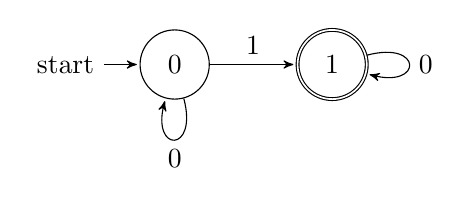
\begin{tikzpicture}[->,>=stealth',shorten >=1pt,auto,node distance=2cm,
        scale = 1,transform shape]

  \node[state,initial] (0) {$0$};
  \node[state,accepting] (1) [right of=0] {$1$};

  \path (0) edge [loop below] node {$0$} (0)
        (0) edge              node {$1$} (1)
        (1) edge [loop right] node {$0$} (1);

\end{tikzpicture}

\subsection{}
This is exactly $0^* \cup 0^*(1 \cup 1(0\cup1)^*0)$, which is clearly \textbf{regular} and accepted by the following DFA:

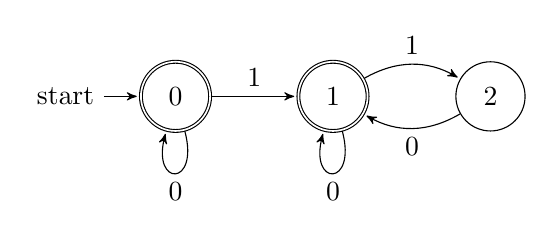
\begin{tikzpicture}[->,>=stealth',shorten >=1pt,auto,node distance=2cm,
        scale = 1,transform shape]

  \node[state,initial,accepting] (0) {$0$};
  \node[state,accepting] (1) [right of=0] {$1$};
  \node[state] (2) [right of=1] {$2$};

  \path (0) edge [loop below] node {$0$} (0)
        (0) edge              node {$1$} (1)
        (1) edge [bend left]  node {$1$} (2)
        (1) edge [loop below] node {$0$} (1)
        (2) edge [bend left]  node {$0$} (1);

\end{tikzpicture}

\subsection{}
We show it is \textbf{not context-free}. Take $p > 0$ arbitrary and put $s = 1^{2^p} = uvxyz$. Suppose we may find some $vxy$ and $i$ such that $uv^ixy^iz = 1^{2^k}$ for some $i \neq 1$. There are two cases. One case is $i = 0$, in which case $k < p$, so $uv^2xy^2z = 2^{p} + 2^{p} - 2^{k}$, which is definitely not in the language. The other case is $i > 1$, in which case $k > p$ and $uv^{2i-1}xy^{2i-1}z = 2^{k} + 2^{k} - 2^{p}$ is also not in the language. Thus, $s$ fails the pumping condition, so the language is not context-free nor regular $\Box$

\subsection{}
This is exactly $(11)^*$ (because 0 is a multiple of 2 as well), so is \textbf{regular} and given by the following DFA:

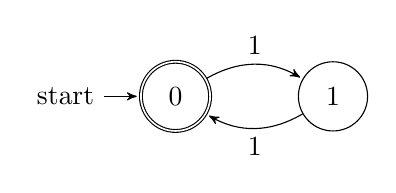
\begin{tikzpicture}[->,>=stealth',shorten >=1pt,auto,node distance=2cm,
        scale = 1,transform shape]

  \node[state,accepting,initial] (0) {$0$};
  \node[state] (1) [right of=0] {$1$};

  \path (0) edge [bend left]  node {$1$} (1)
        (1) edge [bend left]  node {$1$} (0);

\end{tikzpicture}

\subsection{}
This language is \textbf{neither context-free nor regular}. Let $p$ be arbitrary and put
$$s = a^{1+2\left\lceil \frac{3p+1}{2} \right\rceil}b^{\left\lceil \frac{3p+1}{2} \right\rceil}c^p = uvxyz$$
The exponents are chosen so that $j$ is the smallest number satisfying $2j > 3k = 3p$ and $i$ is the smallest number satisfying $i > 2j$. By a \say{section} we mean one of the three contiguous blocks of repeated letters. $vxy$ cannot fall entirely in the first section, since we may then take $uxz$, for which $i \not> 2j$. $vxy$ cannot fall entirely in the second or third sections either, since we may pump $uv^2xy^2z$ to get $i \not> 2j$ and $2j \not> 3k$, respectively. Now suppose $vxy$ crosses the first and second sections. Then $uxz$ is not in the language, since $2j \not> 3z$. Finally, if $vxy$ crosses the second and third sections, $uv^2xy^2z$ does not satisfy $i > 2j$. Then by pumping lemma, the language is not context free and thus also not regular $\Box$

\subsection{}
This language is \textbf{context-free but not regular}. We first show irregularity by pumping lemma. Pick arbitrary $p$ and put $s = a^{2\left\lceil \frac{3p+1}{2} \right\rceil}b^{\left\lceil \frac{3p+1}{2} \right\rceil}c^p = xyz$. Note $s \in E$ since $i \not> 2j$. But since $|xy| \leqslant p$, $y = a^q$ for some $q > 0$. Then $xyyz \in D$, since now $i > 2j > 3k$. Then by pumping lemma the language is not regular. \\
Now we show $E$ is context-free. Denote by $G \subset \Sigma^*$ the set of strings not of the form $a^ib^jc^k$. Define 3 languages: $A = \{a^ib^jc^j \;|\; i \leqslant 2j \} \cup G$, $B = \{a^ib^jc^j \;|\; 2j \leqslant 3k \} \cup G$, $C = \{a^ib^jc^j \;|\; i \leqslant 3k \} \cup G$. We may easily see $E = A \cup B \cup C$. If we can show all of $A,B,C$ are context-free, we are done since the set of context-free languages is closed to finite unions. Briefly, we describe pushdown automata accepting $A$ as follows:
\begin{myindentpar}{1em}
Denote the provided input string by $s$. Push symbol $\$$ onto the stack. If at any point we see a symbol which would indicate $s \in G$, finish reading the input, empty the stack, and accept. (This is easily accomplished by partitioning our state space into the start state and states reachable after reading $a$, $b$, and $c$, respectively, without overlap, then checking each input symbol to make sure we have no transitions $b \to a$, $c \to a$, or $c \to b$.) Otherwise, if we read an $a$, push symbol $a$ to the stack. If we read $c$, do nothing. If we read a symbol $b$ remove $aa$ from the stack, if possible. If it's not possible, finish reading input, empty the stack, and accept. If we run out of input and the top of the stack is $a$, reject. Otherwise, empty the stack and accept.
\end{myindentpar}
We describe a pushdown automata for $B$ as follows:
\begin{myindentpar}{1em}
Denote the provided input string by $s$. Push symbol $\$$ onto the stack. If at any point we see a symbol which would indicate $s \in G$, finish reading the input, empty the stack, and accept. Otherwise, if we read $a$ do nothing. If we read a $b$, push symbols $bb$ to the stack. If we read a symbol $c$ remove $bbb$ from the stack, if possible. If it's not possible, finish reading input, empty the stack, and accept. If we run out of input and the top of the stack is $b$, reject. Otherwise empty the stack and accept.
\end{myindentpar}
Finally we describe a pushdown automata for $C$:
\begin{myindentpar}{1em}
Denote the provided input string by $s$. Push symbol $\$$ onto the stack. If at any point we see a symbol which would indicate $s \in G$, finish reading the input, empty the stack, and accept. Otherwise, if we read an $a$, push symbol $a$ to the stack. If we read $b$, do nothing. If we read a symbol $c$ remove $aaa$ from the stack, if possible. If it's not possible, finish reading input, empty the stack, and accept. If we run out of input and the top of the stack is $a$, reject. Otherwise empty the stack and accept.
\end{myindentpar}
Since all of $A,B,C$ are accepted by pushdown automata, they are context-free and we are done $\Box$

\end{document}

% List of tex snippets:
%   - tex-header (this)
%   - R      --> \mathbb{R}
%   - Z      --> \mathbb{Z}
%   - B      --> \mathcal{B}
%   - E      --> \mathcal{E}
%   - M      --> \mathcal{M}
%   - m      --> \mathfrak{m}({#1})
%   - normlp --> \norm{{#1}}_{L^{{#2}}}
